In this chapter we introduce a technique for improving the scalability of safety validation algorithms for multi-agent systems. We first describe the problem of exponential growth of states and disturbances with respect to the number of adversarial entities. We then show how multi-agent safety validation problems can be decomposed into subproblems each involving the system interacting with a subset of the adversaries. The solution to these subproblems can be recombined using an attention network and a base network to correct for multi-agent interactions. We demonstrate the efficacy of scene decomposition by approximating the distribution over failures of a multi-agent gridworld and T-intersection scenario. 

\section{Motivation}

%todo:cite airspace density commment below
Many of the most exciting use cases for autonomy require the system to interact with large number of other human and non-human agents. An autonomous driving policy must reason about a potentially large number other vehicles, pedestrians, cyclists, and traffic control systems, each with a wide variety of possible behaviors. Similarly, autonomous aircraft will soon have to navigate and avoid collisions in an increasingly dense airspace.

Many of the challenges for safety validation are exacerbated when the environment contains multiple interacting agents. The dimensionality of both the disturbance and state space grows with each new agent in the environment. The search over disturbance trajectories, state-dependent policies, or the state space itself can quickly become intractable. As a probability, failures may be more or less likely with more agents, but the fraction of the disturbance trajectory space that leads to a failure will likely decrease due to the dramatic increase in the size of the disturbance trajectory space. 

As an example, consider the $5 \times 5$ adversarial gridworld problem depicted in \cref{fig:ch6_fullg} where an ego agent (blue) tries to avoid two adversarial agents (orange and red).  Each agent has a 2D position and four possible actions so the state space and disturbance space both grow exponentially with the number of agents. In this case, a failure occurs when all agents overlap on the same state, so failures become less likely with the number agents. Value iteration is tractable on this problem with two adversaries (which is why we include it as a test case), but becomes challenging with \num{3} agents and intractable with more.

The curse of dimensionality is a well known problem in multi-agent systems and is often solved by decomposing the problem into simpler problems that are tractable and then recombining the solutions. In this chapter we develop a technique for decomposing and recombining safety validation problems. The basic idea is to identify a natural decomposition of the state space that reduces the full problem into a set of subproblems that can be solved individually. For example, the gridworld with two adversaries can be decomposed into two gridworlds, each with a single adversary (as shown in \cref{fig:ch6_subg1,fig:ch6_subg2}). Then, to solve the full problem we learn how to combine the subproblem solutions instead of solving the problem from scratch. The solution to the full problem may not be a simple combination of the subproblem solutions so we simultaneously learn a correction factor. 

For this procedure to be successful, however, we need the subproblem solutions to confer some benefit to the solution of the full problem. In the case of the gridworld example, the subproblem solutions will suggest that it is beneficial to move toward the ego to cause failure. This insight will likely aid the adversary when solving the full problem.

In the next section we formalize the decomposition and highlight some potential efficiencies. We then demonstrate that combining the subproblems can be cast as a transfer learning problem and we apply a known transfer learning algorithm to solve it. 


\begin{figure*}
    \centering
    \begin{subfigure}[b]{0.25\textwidth}
        \centering
        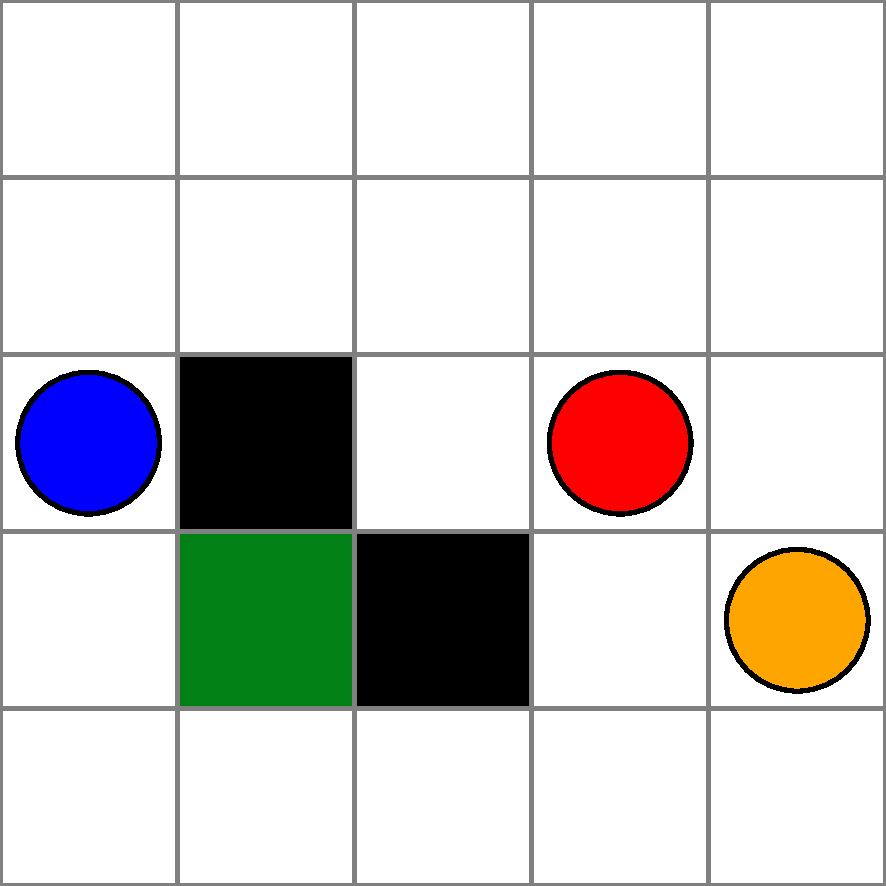
\includegraphics[width=\textwidth]{figures/problem_decomposition/g.pdf}
        \caption{Full problem.}
        \label{fig:ch6_fullg}
    \end{subfigure}
    \hfill
    \begin{subfigure}[b]{0.25\textwidth}
        \centering
        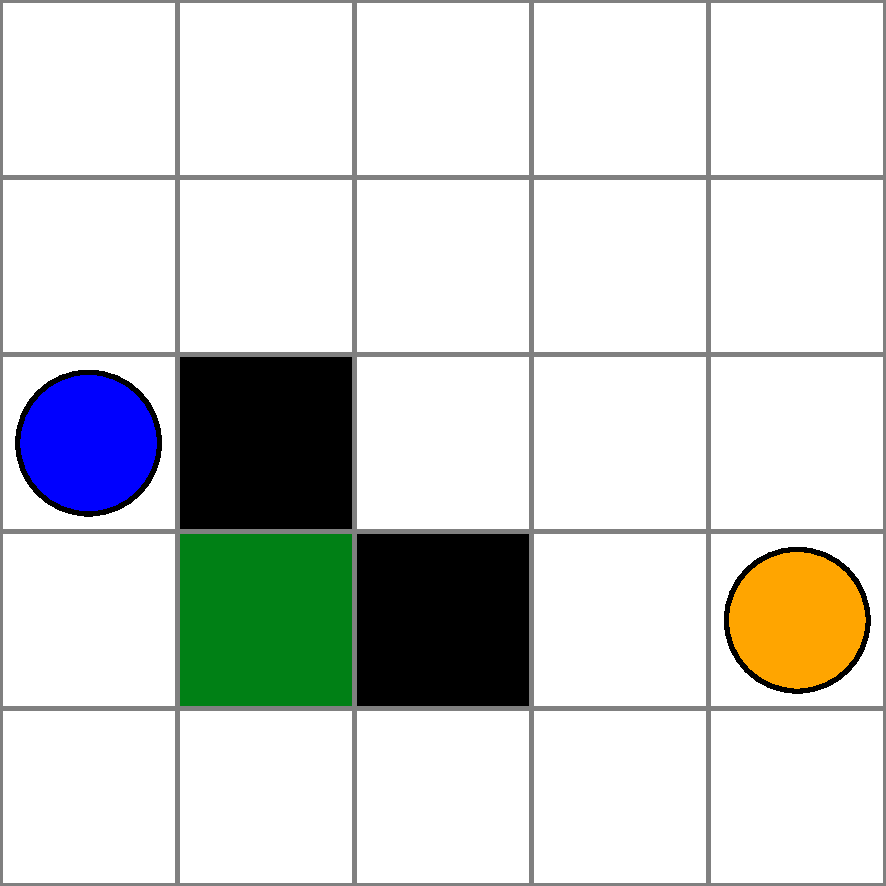
\includegraphics[width=\textwidth]{figures/problem_decomposition/g_sub1.pdf}
        \caption{Subproblem 1}
        \label{fig:ch6_subg1}
    \end{subfigure}
    \hfill
    \begin{subfigure}[b]{0.25\textwidth}
        \centering
        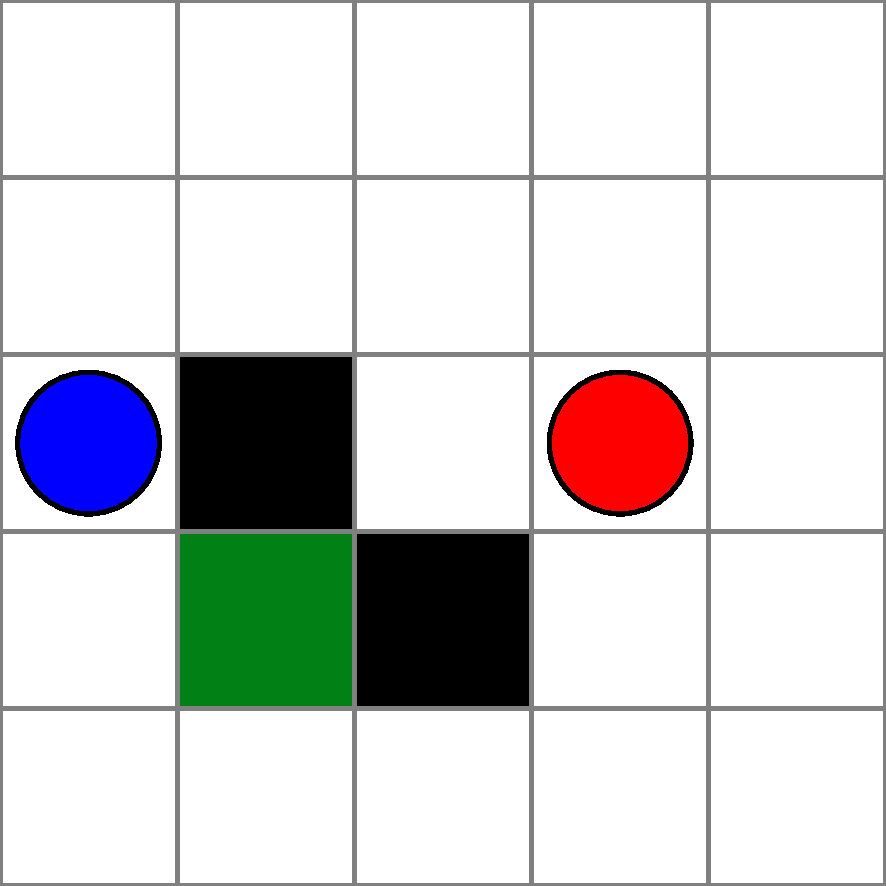
\includegraphics[width=\textwidth]{figures/problem_decomposition/g_sub2.pdf}
        \caption{Subproblem 2.}
        \label{fig:ch6_subg2}
    \end{subfigure}
    \caption{Example decomposition of the gridworld with two adversaries.}
    \label{fig:adv_gridworld_decomp}
\end{figure*}

\section{Decomposition and Fusion}
In this section we describe the process of problem decomposition and identify situations where subproblems are identical. We then introduce the attend, adapt, and transfer algorithm that automatically learns how to combine the subproblem solutions while learning a correction factor. 

\subsection{Problem Decomposition}
The goal of state-space decomposition is to identify a set of subspaces that each represent a similar, but smaller, version of the full problem. We denote the state space of the $i$th subproblem $S^{(i)}$ and the disturbance space $X^{(i)}$. The state $s^{(i)} \in S^{(i)}$ contains the components of $s$ that are associate with the $i$th subproblem and similarly for the disturbance $x^{(i)}$. A crucial constraint on the choice of decomposition is the ability to simulate transitions of the subproblems
\begin{equation}
    s_{t+1}^{(i)} \sim P( s^{(i)} \mid s_t^{(i)}, x_t^{(i)} ) \text{.}
\end{equation}

In the gridworld example, if we choose a decomposition where the state space consists only of the horizontal component of each agent, it is not clear how we would choose a transition model that is faithful to the original problem. Instead, if we choose a decomposition where the state space is the position of the ego and one adversary, and the disturbance space is the disturbance space of that adversary then we have reduced the problem a single-adversary gridworld which we know how to simulate. Indeed, in multi-agent problems a natural decomposition usually consists of the state spaces from a subset of of the agents. 

In some cases, multiple subproblems will reduce to the same problem and only one solution will be required. For example, suppose we wish to solve for the probability of failure at each state in a gridworld with $N$ adversarial agents. If we decompose it into $N$ gridworlds (each with the ego and one adversary), then each subproblem is identical (assuming the ego agent cannot distinguish adversaries). Noticing these overlaps can save a significant amount of computational effort when computing subproblem solutions. The next section describes how to combine subproblem solutions once they are computed. 

\subsection{Solution Fusion}
We now assume that we have decomposed the safety validation problem into $M$ subproblems and obtained a solution $K$ for each. We assume that solution takes the form of a policy or a value function that solves the associated subproblem. For falsification and most-likely failure analysis tasks, $K$ should produce the lowest cost failure trajectories. When approximating the distribution over failures $K$ may estimate the probability of failure at each state or be the distribution over failures of the subproblem. Then, the goal is to use the $M$ subproblems to learn the solution to the full problem 
\begin{equation}
K_{\rm full} = \mathcal{L}(K_1, \ldots, K_M) \label{eq:ch6_solution_fusion}
\end{equation}
with some learning algorithm $\mathcal{L}$. Fortunately, this problem formulation is the same as transfer learning, which has many existing solution techniques~\cite{taylor2009transfer}.

% Intro to A2T
In safety validation, the full problem may contain failure modes that arise from the complex interaction of multiple agents and are therefore not present in the subproblems. The solutions to the subproblems may not contain the needed information for finding failures in the full problem and may even make it more difficult to find failures (an effect known as negative transfer). From these considerations we selected the attend, adapt, and transfer algorithm (A2T)~\cite{rajendran2017attend}. A2T combines solutions using a learned set of attention weights that can minimize negative transfer, and simultaneously learns a new solution from scratch to account for the complexities of the full problem. 

With A2T, the full solution at state $s$ is given by 
\begin{equation}
K_{\rm full}(s) = w_0(s) K_{\rm base}(s) + \sum_{i=1}^M w_i(s) K_i(s^{(i)}) \label{eq:ch6_a2t}
\end{equation}
where $w(s)$ is a state-dependent attention weight and $K_{\rm base}$ is the solution learned from scratch. \cref{eq:ch6_a2t} can be encoded as the network architecture shown in \cref{fig:ch6_A2T_Network}. The state is passed to the base network, the set of subproblem solutions, and an attention network. The base network outputs $K_{\rm base}(s)$ while the subproblem solutions output $K_i(s^{(i)}$. The attention network outputs the attention weights $w_i(s)$ which are combined with $K_{\rm base}$ and $K_i$ to get the full solution $K_{\rm full}(s)$. The parameters in the base network and the attention network can be optimized through backpropagation (as indicated by the dashed lines), using any typical learning algorithm such as DQN or policy gradient methods.

\begin{figure}[!t]
\centering
% TikZ diagram for black-box safety validation problem formulation.
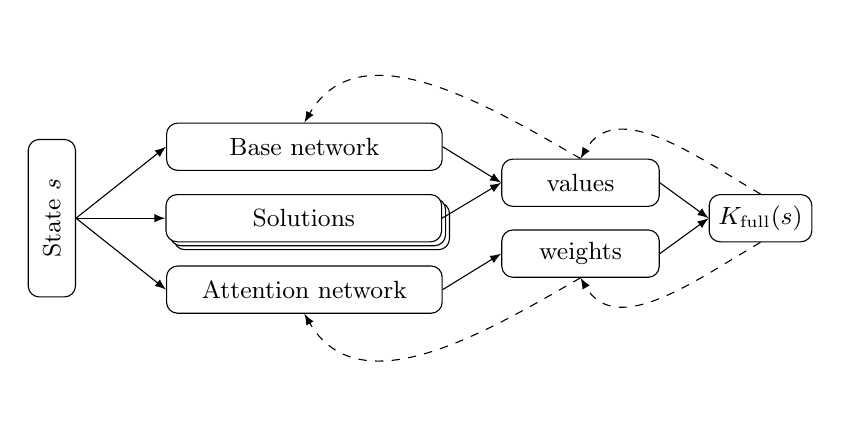
\begin{tikzpicture}
    \tikzstyle{every node}=[font=\small, align=center]
    \tikzset{
        n/.style={draw, rounded corners, minimum height=0.6cm, minimum width = 2cm},
        n2/.style={n, minimum width=3.5cm}
        }
    
    %state 
    \node (state) [n, rotate=90] {\small State $s$};
    
    %base network
    \node (base) [n2, above right of=state, xshift=2.5cm, yshift = 0.2cm] {Base network};
    
    %Solutions
    \node (solutionsback1) [n2, right of=state, xshift=2.3cm, yshift=-0.1cm] {};
    \node (solutionsback2) [n2, fill=white, right of=state, xshift=2.25cm, yshift=-0.05cm] {};
    \node (solutions) [n2, fill=white, right of=state, xshift=2.2cm] {Solutions};
    
    %weights
    \node (attn) [n2, below right of=state, xshift=2.5cm, yshift=-0.2cm] {Attention network};
    

    \node (values) [n, below right of=base, xshift=2.8cm, yshift = 0.25cm] {values};
    
     \node (weights) [n, above right of=attn, xshift=2.8cm, yshift = -0.25cm] {weights};
     
     \node (pfail) [n, minimum width = 0.5cm, right of=state, xshift=8cm] {$K_{\rm full}(s)$};
    

    \draw[-latex] (state.south) -- (base.west);
    \draw[-latex] (state.south) -- (solutions.west);
    \draw[-latex] (state.south) -- (attn.west);
    
    \draw[-latex] (base.east) -- (values.west);
    \draw[-latex] (solutions.east) -- (values.west);
    \draw[-latex] (attn.east) -- (weights.west);
    
    \draw[-latex] (weights.east) -- (pfail.west);
    \draw[-latex] (values.east) -- (pfail.west);
    
    
    % backprop
    
    \draw [dashed, -latex] (weights.south) to [out=-150,in=-60] (attn.south);
    \draw [dashed, -latex] (pfail.south) to [out=-150,in=-60] (weights.south);
    \draw [dashed, -latex] (values.north) to [out=150,in=60] (base.north);
    \draw [dashed, -latex] (pfail.north) to [out=150,in=60] (values.north);
\end{tikzpicture}
\caption{The A2T network. }
\label{fig:ch6_A2T_Network}
\end{figure}


\section{Experiments}

In this section we perform experiments to investigate the benefit of problem decomposition for approximating the distribution over failures. As discussed in \cref{ch5}, to approximate the distribution over failures we need to estimate the probability of failure at each state. The solutions $K_i(s)$ will represent the probability of failure for each disturbance from state $s$. 

In the first experiment we use the gridworld scenario with two adversaries because it can be solved with exact value iteration. Having the ground truth allows us to compare estimates of the probability of failure with and without the subproblem solutions. In the second experiment we solve for the distribution over failures in the T-intersection with \num{4} adversaries and show it outperforms our baseline approaches. Lastly, we demonstrate that the attention network may also lend a degree of interpretability to the safety validation results. 

\subsection{Adversarial Gridworld Example}

The goal of this experiment is to compare the estimates of the probability of failure between a basic neural network and an A2T network that uses estimates of the probability of failure from decomposed subproblems. To make the comparison, we use value iteration to obtain the ground truth $P_{\rm fail}(s)$ of a $5 \times 5$ gridworld with \num{2} adversaries and an expert ego policy. 

As previously described, the gridworld can be decomposed into two identical gridworlds each with a single adversary (\cref{fig:adv_gridworld_decomp}). We solve for the probability of failure for each state and disturbance of the single-adversary problem $P^{\rm sub}_{\rm fail}(s^{(i)}, x^{(i)})$ using exact value iteration. The A2T estimate of the probability of failure is then given by
\begin{equation}
\begin{split}
    P^{\rm A2T}_{\rm fail}(s, x) = w_0(s) P_{\rm fail}^{\rm base}(s, x) &+ \sum_{i=1}^2 w_i(s) P^{\rm sub}_{\rm fail}(s^{(i)}, x^{(i)}) \\
    &+ w_3(s) P^{\rm sub}_{\rm fail}(s^{(1)}, x^{(1)})P^{\rm sub}_{\rm fail}(s^{(2)}, x^{(2)})
\end{split}
\end{equation}
where we included the last term to help model the conjunctive nature of the failure mode of the full problem. 

The attention network has a single hidden layer with \num{32} units and has a softmax layer at the output to normalize the weights. The base network has two hidden layers with \num{64} and \num{32} units and relu activations. The base network has sigmoid activations on the last layer to ensure the output is bounded in $(0,1)$. The A2T network is compared against a neural network with same architecture as the base network. Both networks were trained using our version of DQN for $P_{\rm fail}$ estimation (see \cref{ch5}). We trained for \num{1e5} steps with the ADAM optimizer and a learning rate of \num{1e-3}. 

During training we periodically computed the mean square log error between the estimate and the ground truth and plotted the results in \cref{fig:ch6_adv_gridworld_training}. We first notice that the A2T network reaches its lowest error more quickly than the basic network, but more importantly, remains close to this error for the rest of training, likely because it is near a local minimum. The basic network initially reduces in error but eventually goes unstable and does not converge to a minimum. The use of subproblem solutions speeds up the training process and appears to improve the training stability as well. We now perform some experiments on the T-intersection problem to more fully demonstrate the problem decomposition technique.

\begin{figure}
        \centering
        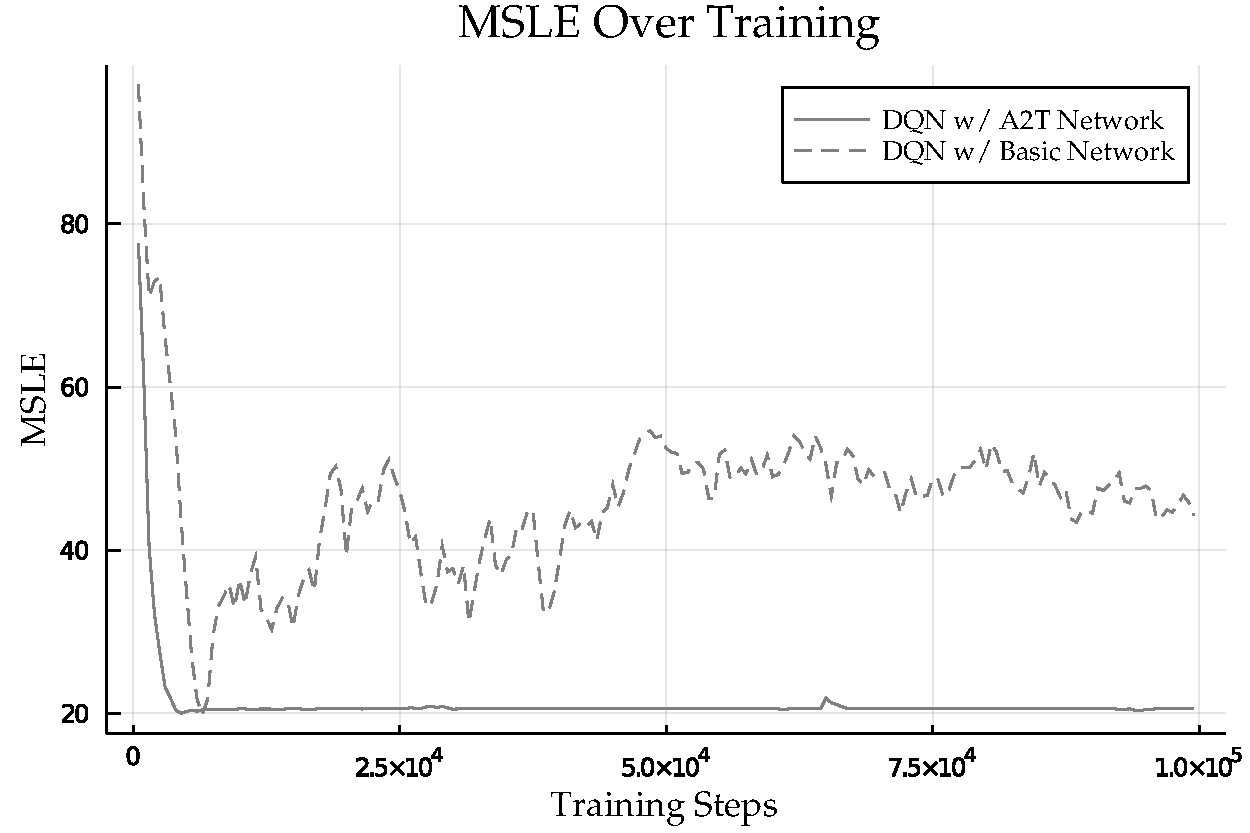
\includegraphics[width=\textwidth]{figures/problem_decomposition/training_comparison.pdf}
        \caption{Training comparison between A2T and basic network.}
        \label{fig:ch6_adv_gridworld_training}
\end{figure}


\subsection{T-Intersection Scenario}

We now solve for the failure distribution of the T-intersection autonomous driving scenario with five interacting agents. If we were to discretize the state space of the full problem (using the same discretization as in \cref{sec:ch5_Tint}) we would end up with over \num{1e14} states and \num{2401} actions. Instead we apply problem decomposition to construct subproblems that each consist of one of the adversaries and the ego vehicle. The result is two unique subproblems, one with the adversary coming from the left, and one with adversary coming from the right. We solve both of those problems using DQN and the same architecture described in \cref{sec:ch5_Tint}. We combine the solutions with an A2T architecture with a base and attention network each with two hidden layers of \num{128} and \num{32} units and relu activations. To handle the explosion in actions, we make the simplifying assumption that only one adversary can have a disturbance at a time which reduces the action space to \num{25} actions.  

% architecture and raining details
The A2T network to approximate the probability of failure was trained over \num{3e5} steps with a learning rate of \num{1e-3}. The resulting proposal distribution was compared to the same baselines as \cref{sec:ch5_expr}. For each episode the initial condition of each adversary was sampled with the position in [\SI{0}{m}, \SI{45}{m}] and the velocity in  [\SI{5}{m}, \SI{20}{m/s}]. The ego vehicle was initialized with a position in [\SI{10}{m}, \SI{35}{m}] and velocity in [\SI{10}{m}, \SI{20}{m/s}]. Any initial condition that had a collision without any disturbance (due to overlapping initialization for example) was skipped in the analysis. Additionally when computing the probability of failure we removed samples that had too large of an importance sample weight to reduce the variance of the estimates. 

% Discussion of results
The failure rates on the log-likelihood of the failures are reported in \cref{tab:ch6_5car_results} and the probability of failure is plotted in \cref{fig:ch6_5car_pfail_estimation}. First, we note that the probability of failure was sufficiently low that we never observed a failure event for Monte Carlo sampling in the allotted trials. Uniform sampling of the disturbances found a similar number of failures as the cross entropy method but had significantly lower log-likelihood. As such uniform sampling dramatically underestimates the probability of samples and is below the axis of the plot. The cross entropy method was an improvement but still had a low prediction until many failures were observed. The estimate of the probability of failure using A2T performed the best across all categories and produced a good estimate of the probability of failure from only a few samples.

% Discussion of failure modes and attention weights
Two example failures are shown in \cref{fig:five_car_collision1,fig:five_car_collision2} where the blue circles indicated the associated attention weight. In the first collision, the ego vehicle calculates that it can make a turn in front of the leading vehicle on the right. That vehicle, however, speeds up unexpectedly and causes a collision. During the first half of the trajectory, the adversary is computing the probability of failure based on both agents on the right, likely meaning that both agents have a possibility of causing a collision. By the time collision is imminent, the adversary has focused on the vehicle that causes the collision. The attention weights might be some indication of which adversaries are most likely to cause a collision. The second collision starts out similar to thee first, but by timestep \num{8} the attention network is focused on the trailing left adversary which is the vehicle ultimately responsible for the collision. When the collision is imminent, the attention goes back to a vehicle on the right. It may be the case that the vehicle on the right could also cause a collision so the network has conflated the two estimates. 

Finding failures in a complex driving scenario with multiple interacting agents is challenging due to the large state and action spaces. We have successfully applied problem decomposition and recombination with A2T to discover the most likely failure modes estimate the probability of failure. 

\begin{table}
    \centering
    \caption{5-car Results}
    \label{tab:ch6_5car_results}
    \begin{tabular}{@{}lll@{}} 
        \toprule
        \textbf{Method} & \textbf{Failure Rate} & \textbf{Log Likelihood}\\
        \midrule
        Monte Carlo & \num{0.0} \pm \num{0.0} &  - \\
        Uniform sampling & \num{0.031} \pm \num{0.005} & \num{-173.01} \pm \num{42.925} \\
        Cross entropy method & \num{0.035} \pm \num{0.006} & \num{-82.672} \pm \num{7.342} \\
        DQN + A2T & \num{0.081} \pm \num{0.009} & \num{-19.938} \pm \num{7.317} \\
        \bottomrule
    \end{tabular}
\end{table}

\begin{figure}
        \centering
        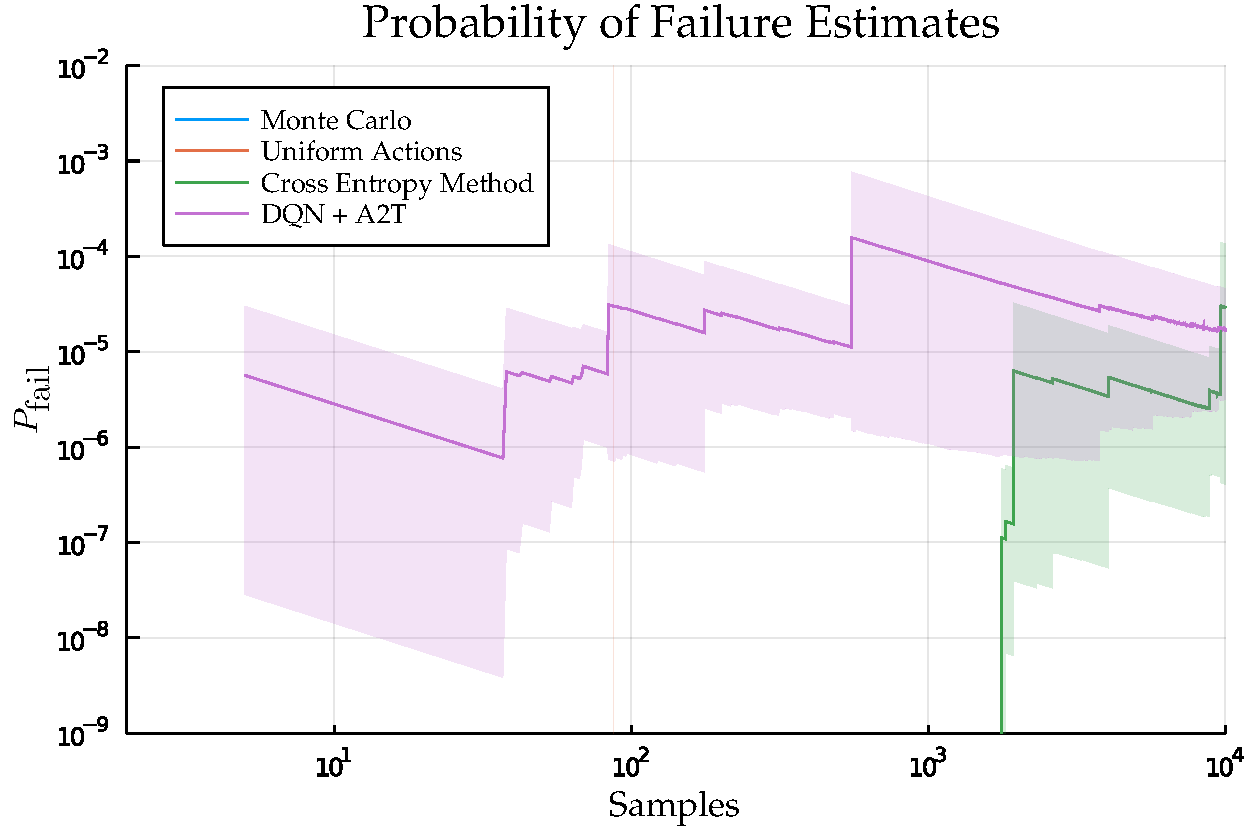
\includegraphics[width=\textwidth]{figures/problem_decomposition/pfail_5car.pdf}
        \caption{Comparison of techniques for $P_{\rm fail}$ estimation for the 5-car T-intersection scenario.}
        \label{fig:ch6_5car_pfail_estimation}
\end{figure}

\begin{figure}
    \centering
   \begin{subfigure}[t]{0.7\textwidth}
        \centering
        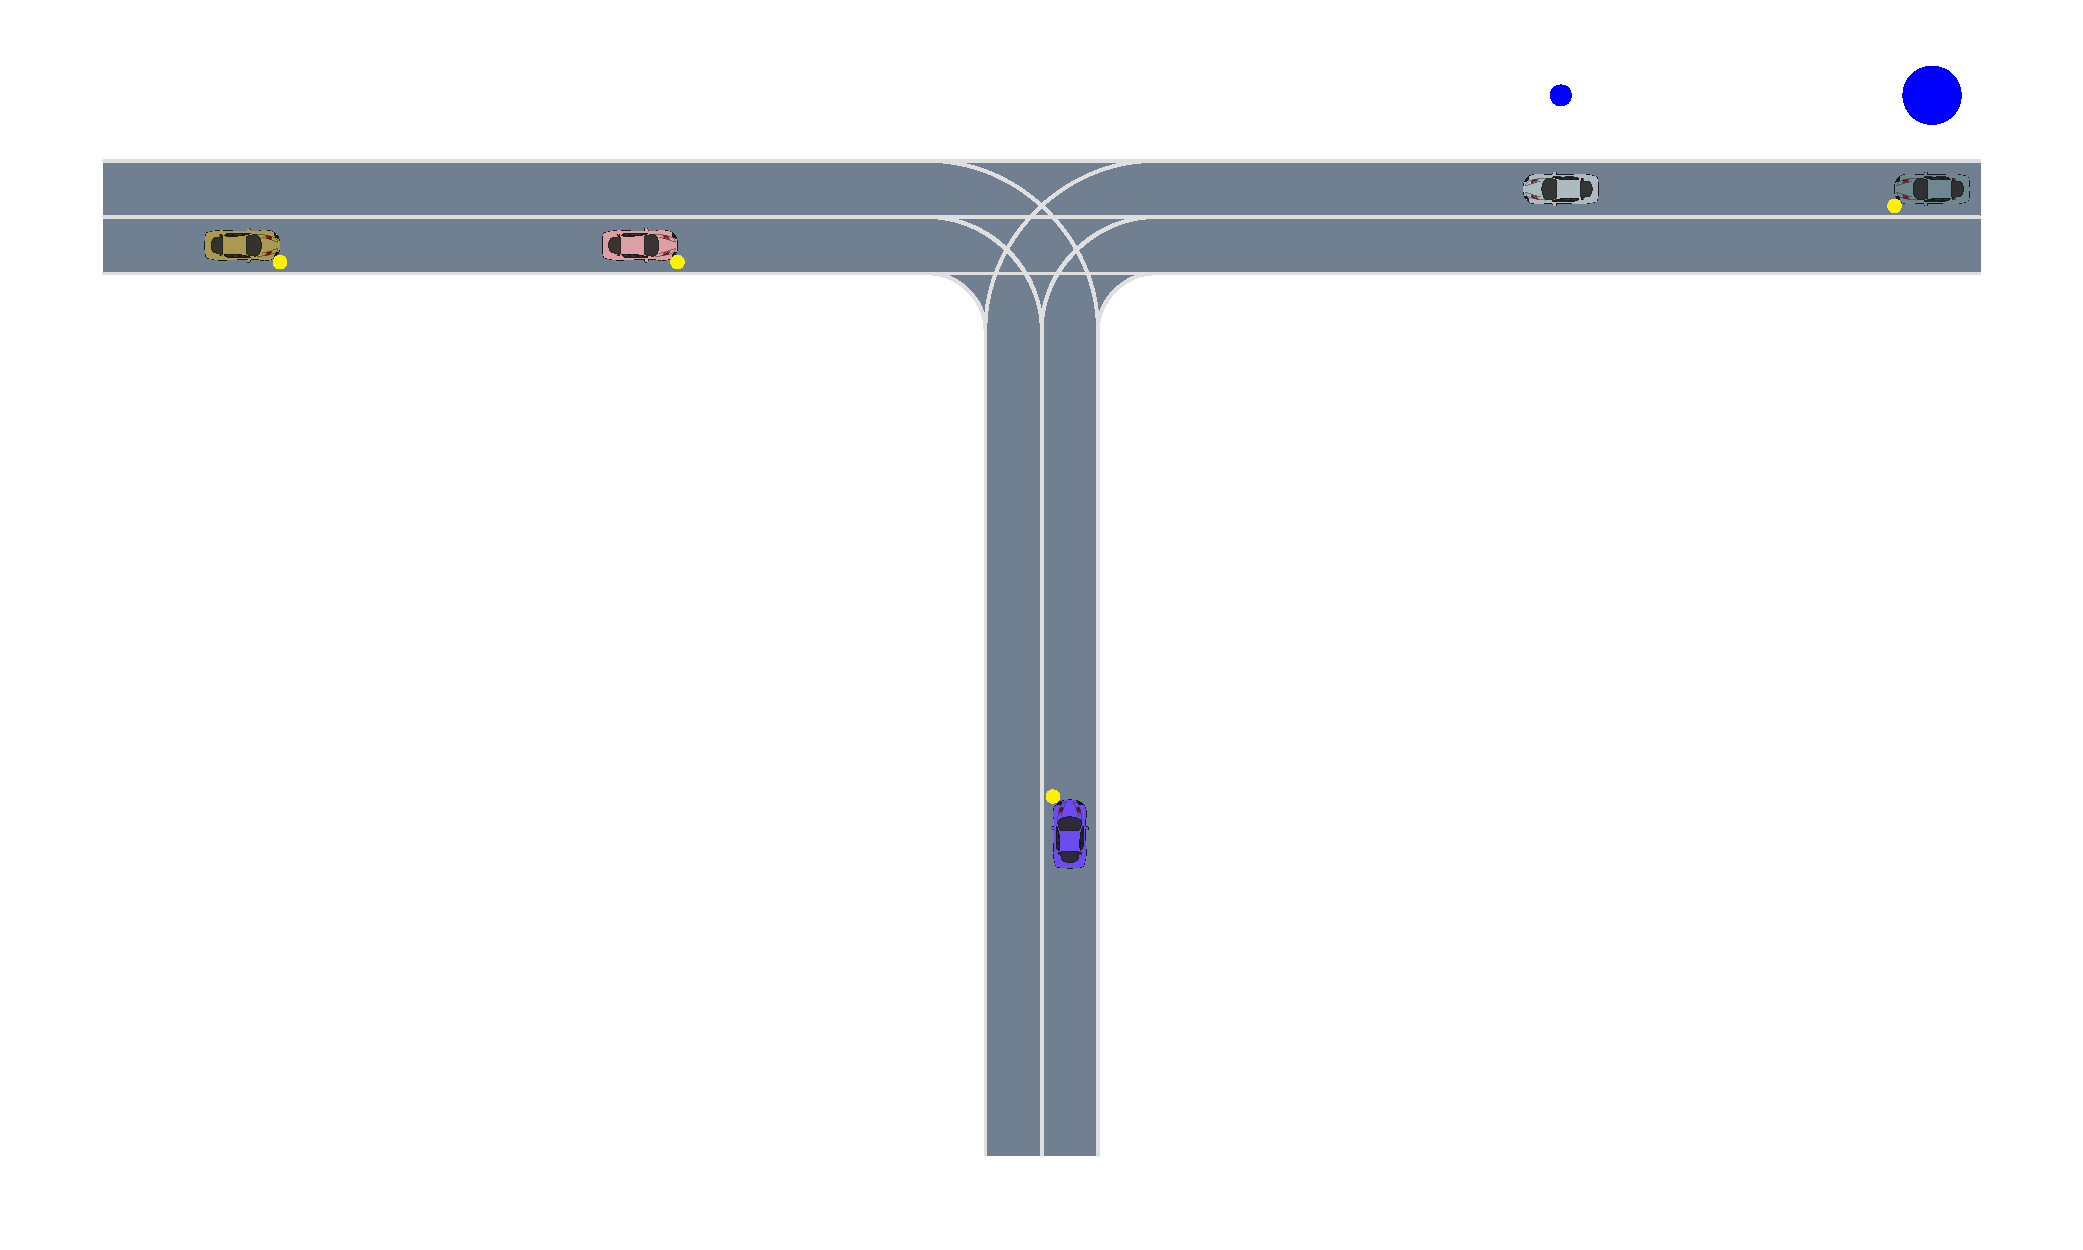
\includegraphics[width=\textwidth, trim={2cm 5cm 1cm 0},clip]{figures/problem_decomposition/f1_1.pdf}
    \end{subfigure}
    \begin{subfigure}[t]{0.7\textwidth}
        \centering
        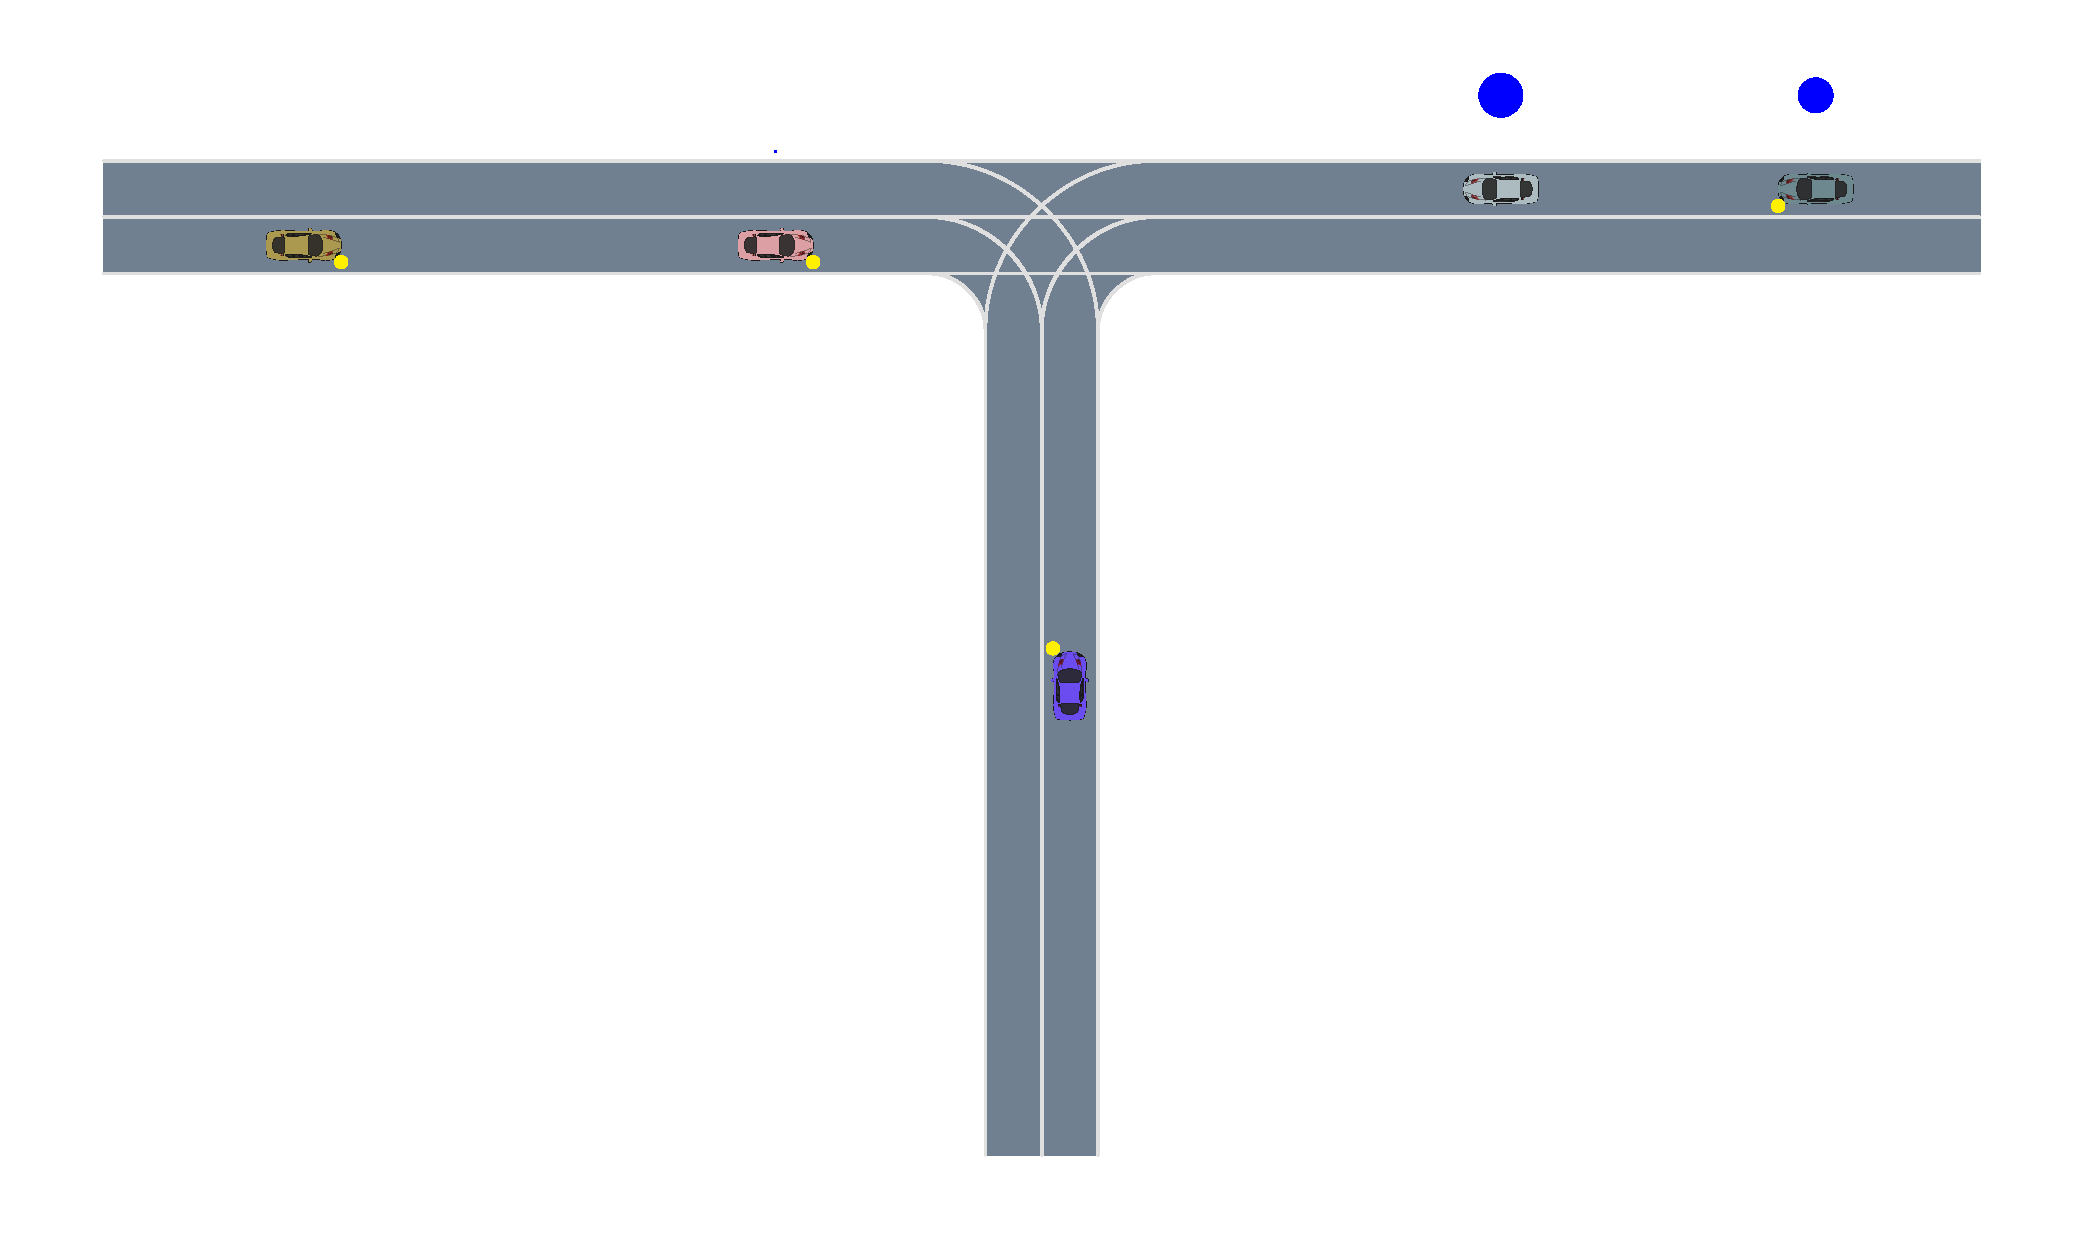
\includegraphics[width=\textwidth, trim={2cm 5cm 1cm 0},clip]{figures/problem_decomposition/f1_4.pdf}
    \end{subfigure}
    \begin{subfigure}[t]{0.7\textwidth}
    \centering
    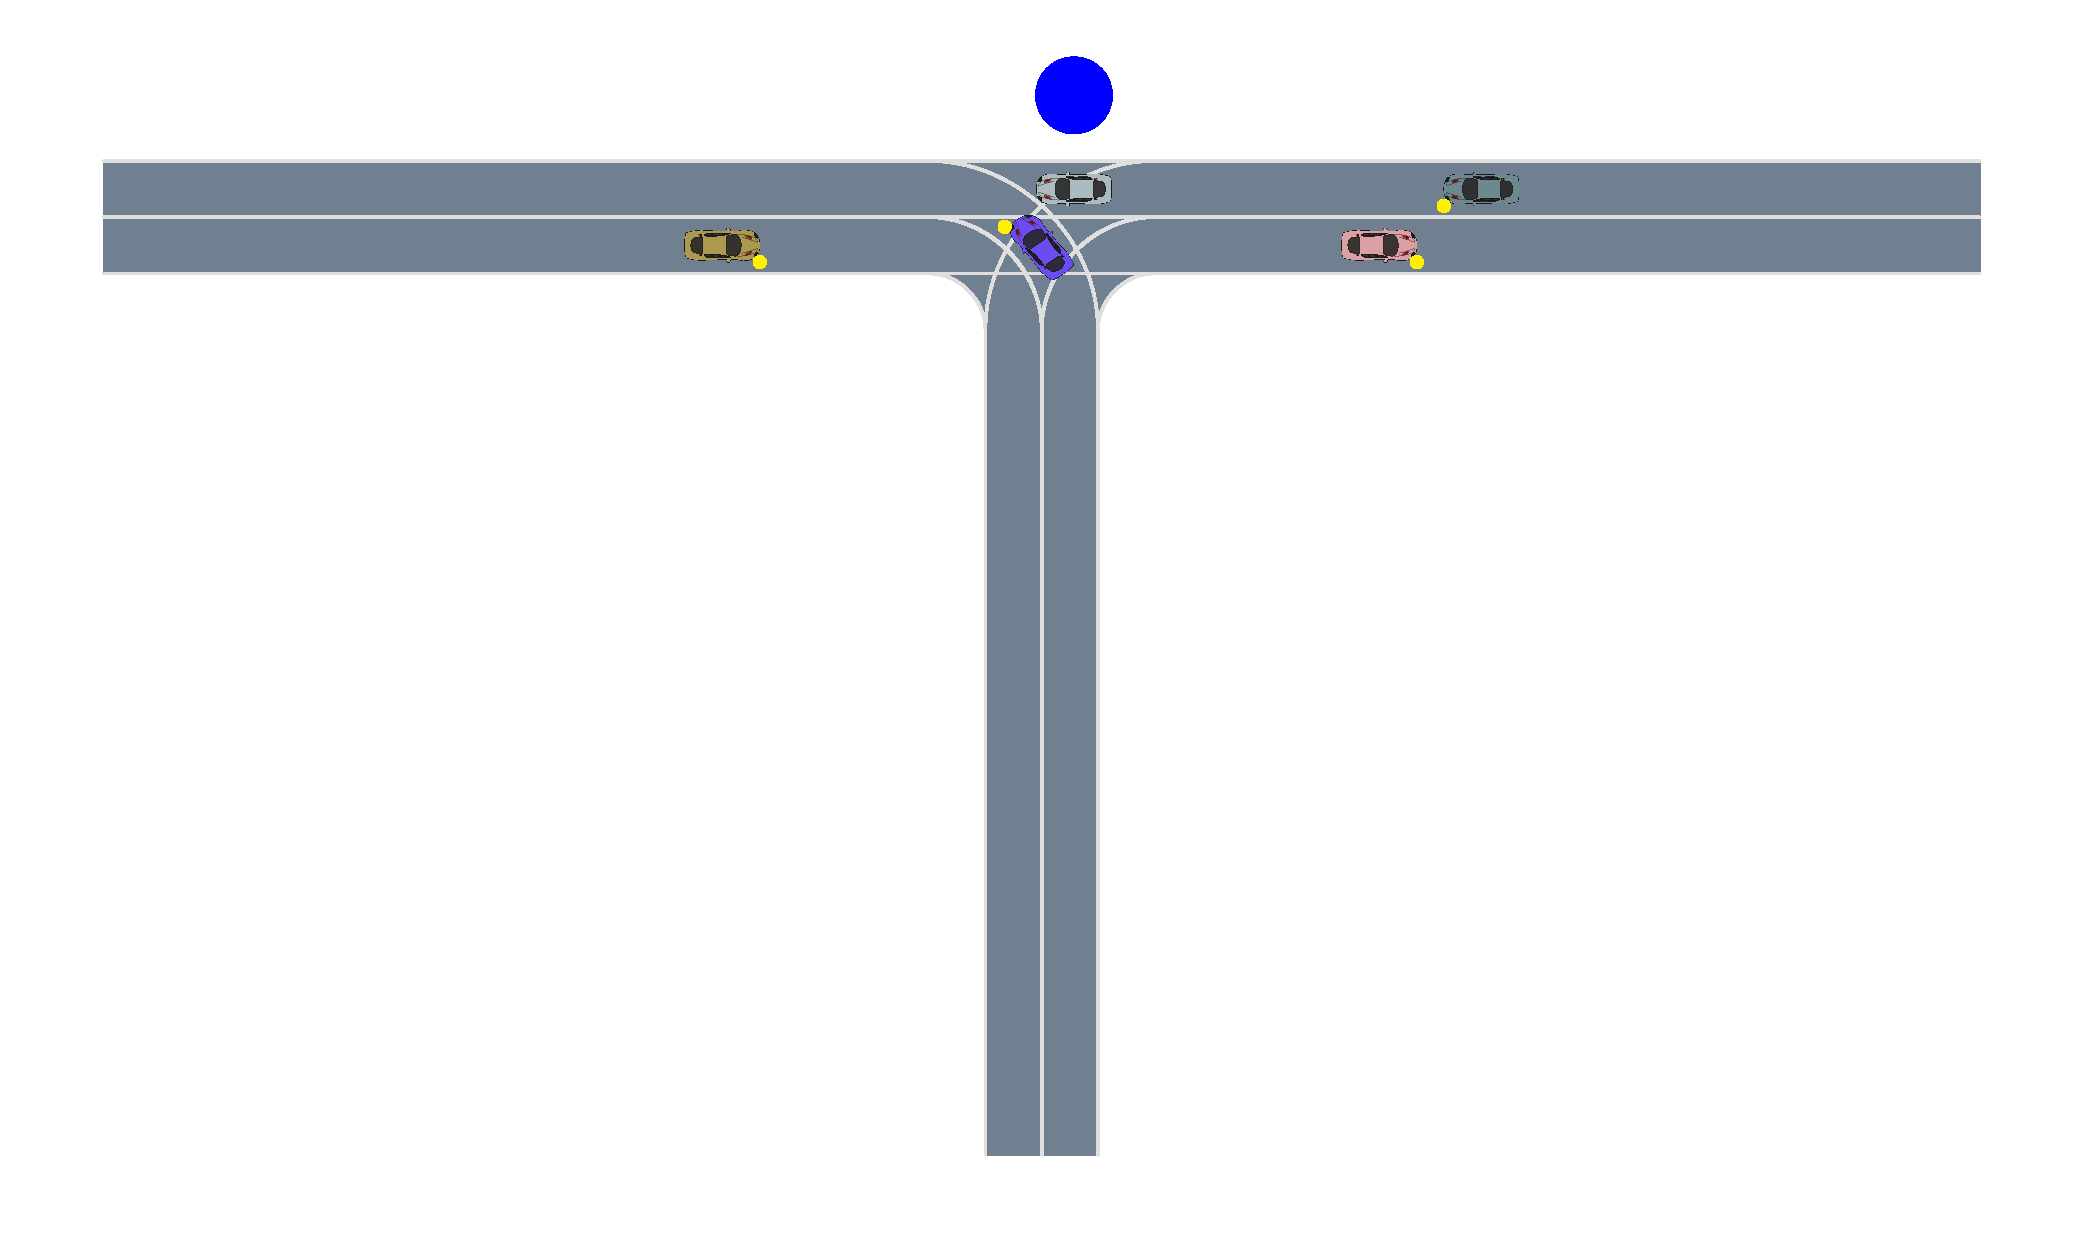
\includegraphics[width=\textwidth, trim={2cm 5cm 1cm 0},clip]{figures/problem_decomposition/f1_18.pdf}
\end{subfigure}
    \caption{Collision in 5-car scenario at timesteps $t=[1,4,18]$}
    \label{fig:five_car_collision1}
    \vspace{-0.2in}
\end{figure}


\begin{figure}
    \centering
   \begin{subfigure}[t]{0.7\textwidth}
        \centering
        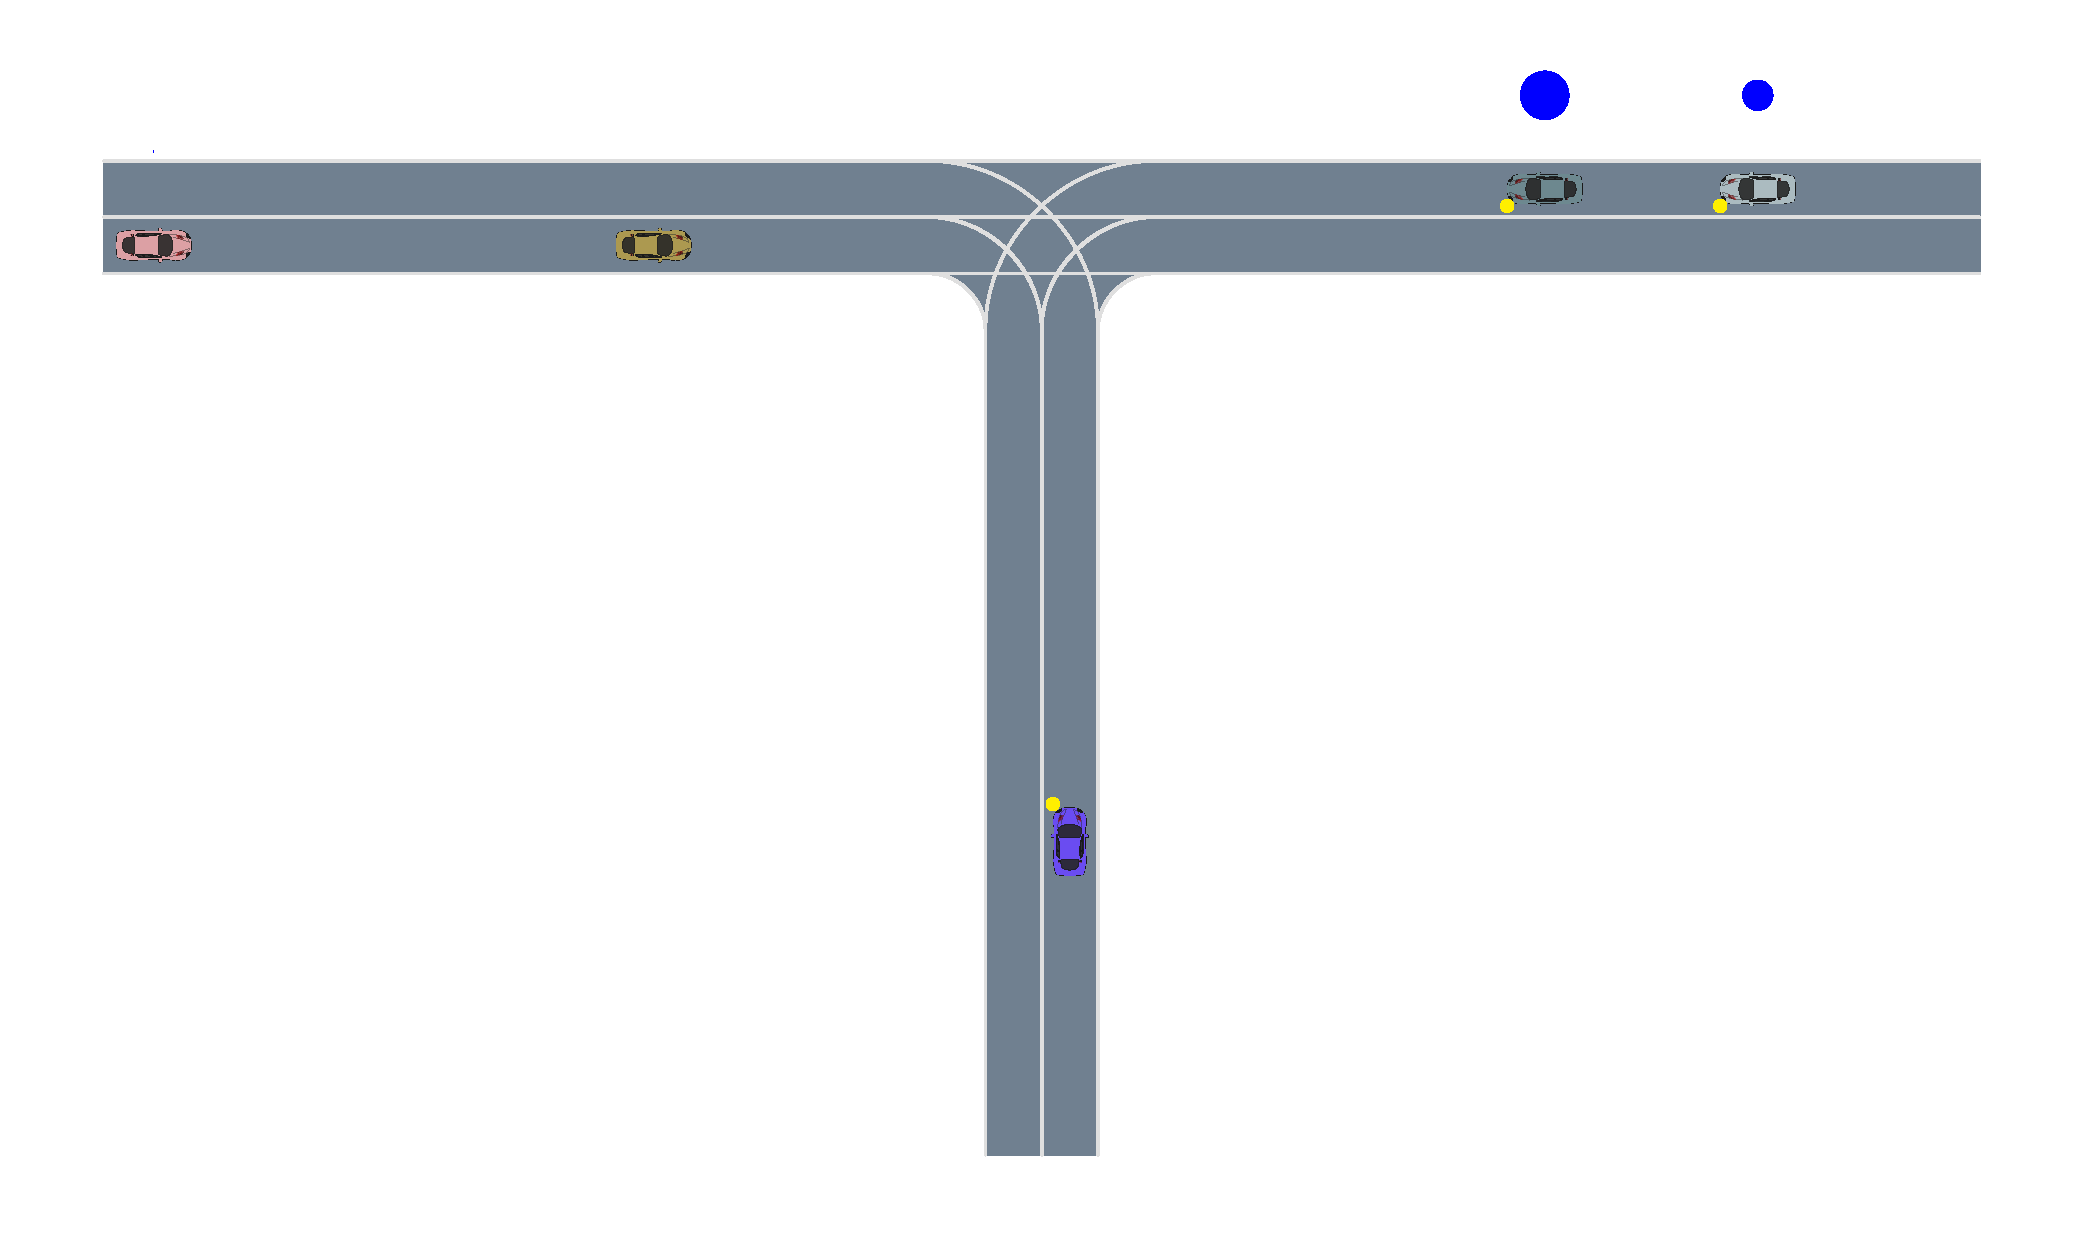
\includegraphics[width=\textwidth, trim={2cm 5cm 1cm 0},clip]{figures/problem_decomposition/f2_1.pdf}
    \end{subfigure}
    \begin{subfigure}[t]{0.7\textwidth}
        \centering
        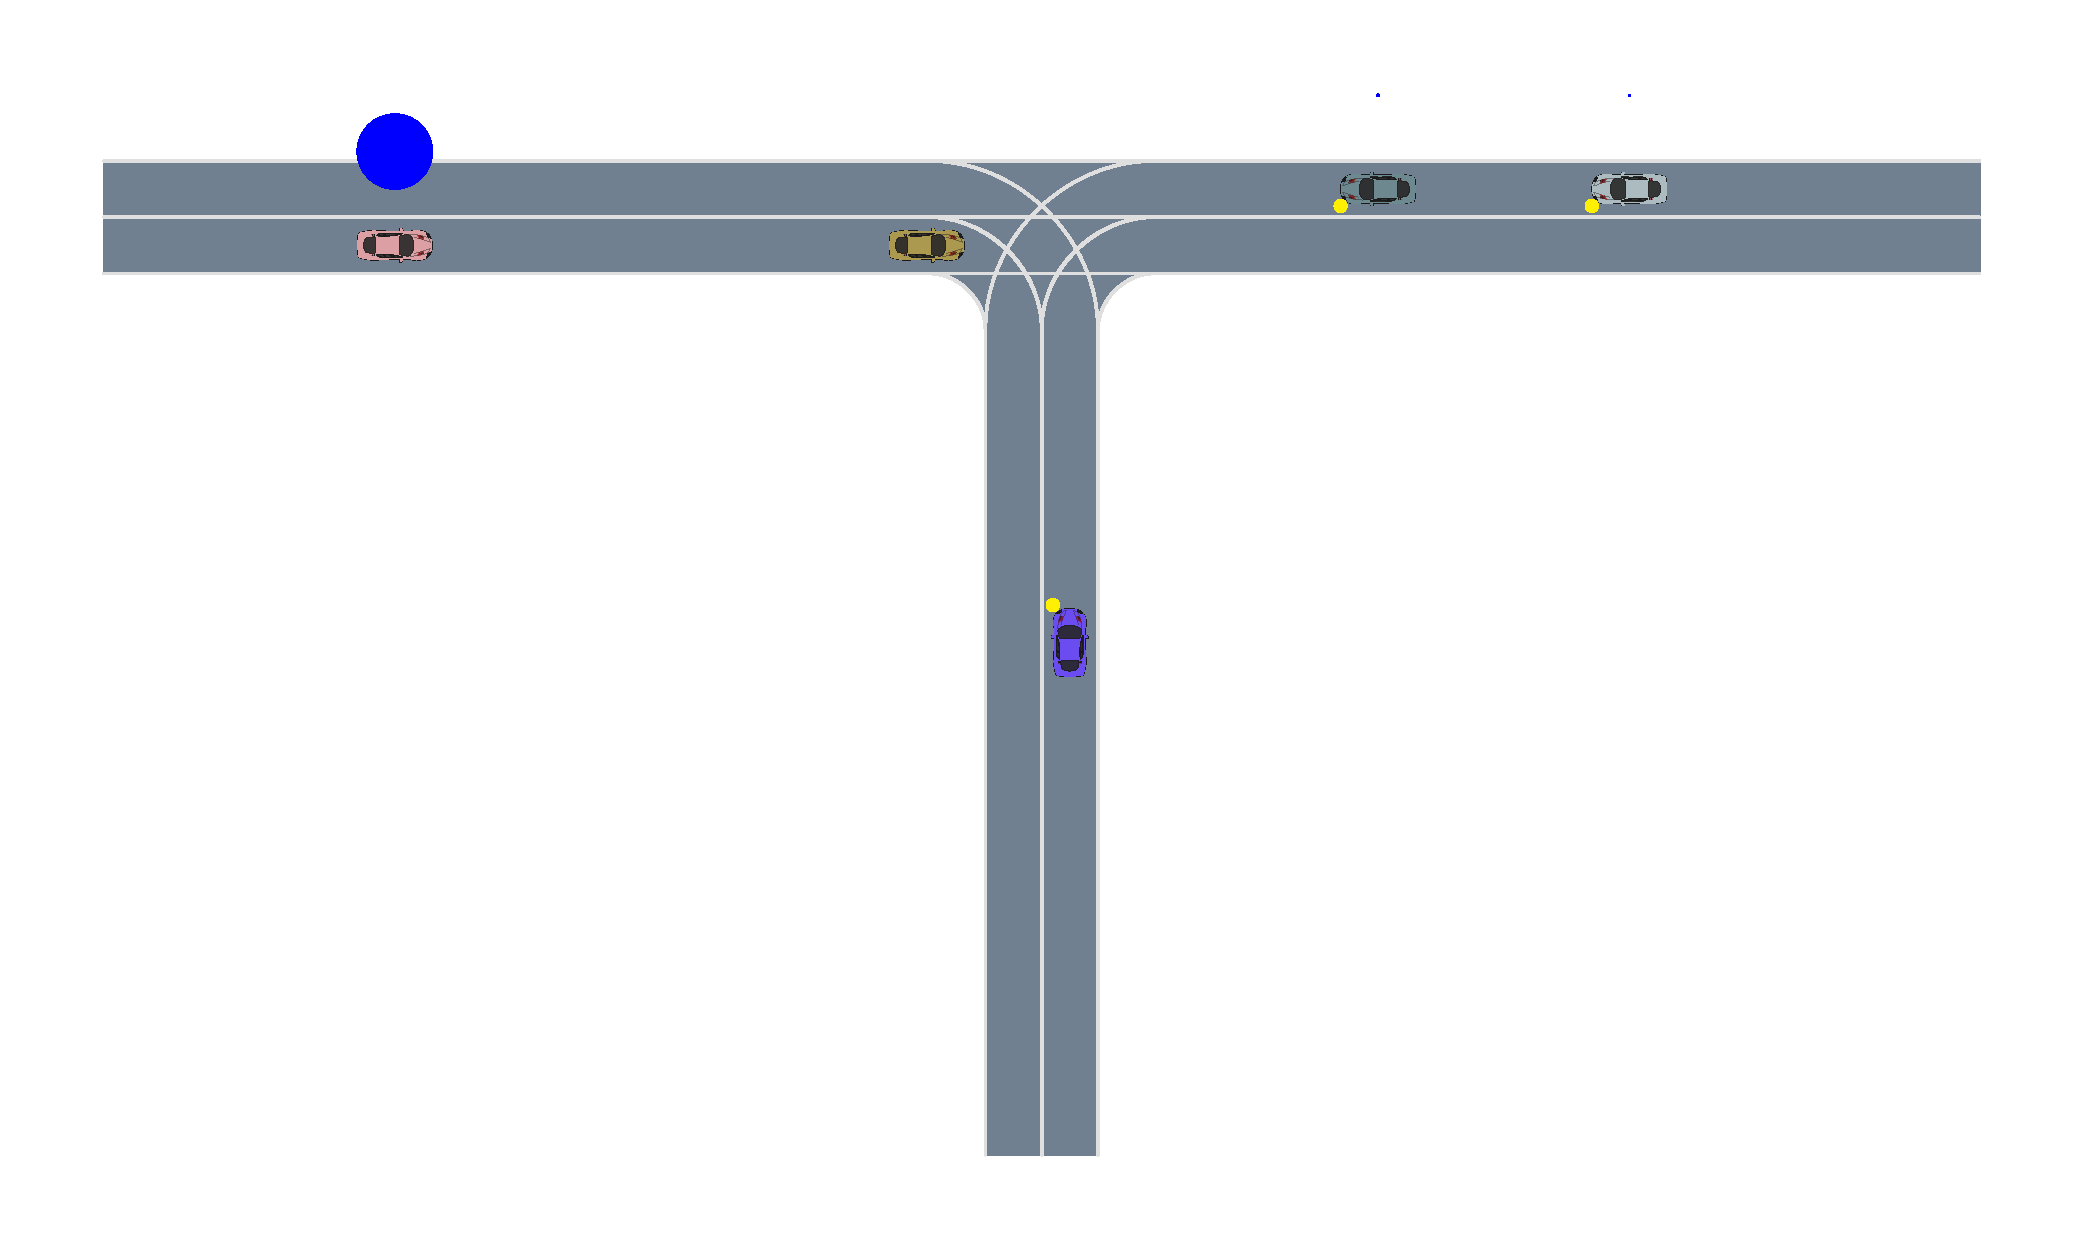
\includegraphics[width=\textwidth, trim={2cm 5cm 1cm 0},clip]{figures/problem_decomposition/f2_8.pdf}
    \end{subfigure}
    \begin{subfigure}[t]{0.7\textwidth}
    \centering
    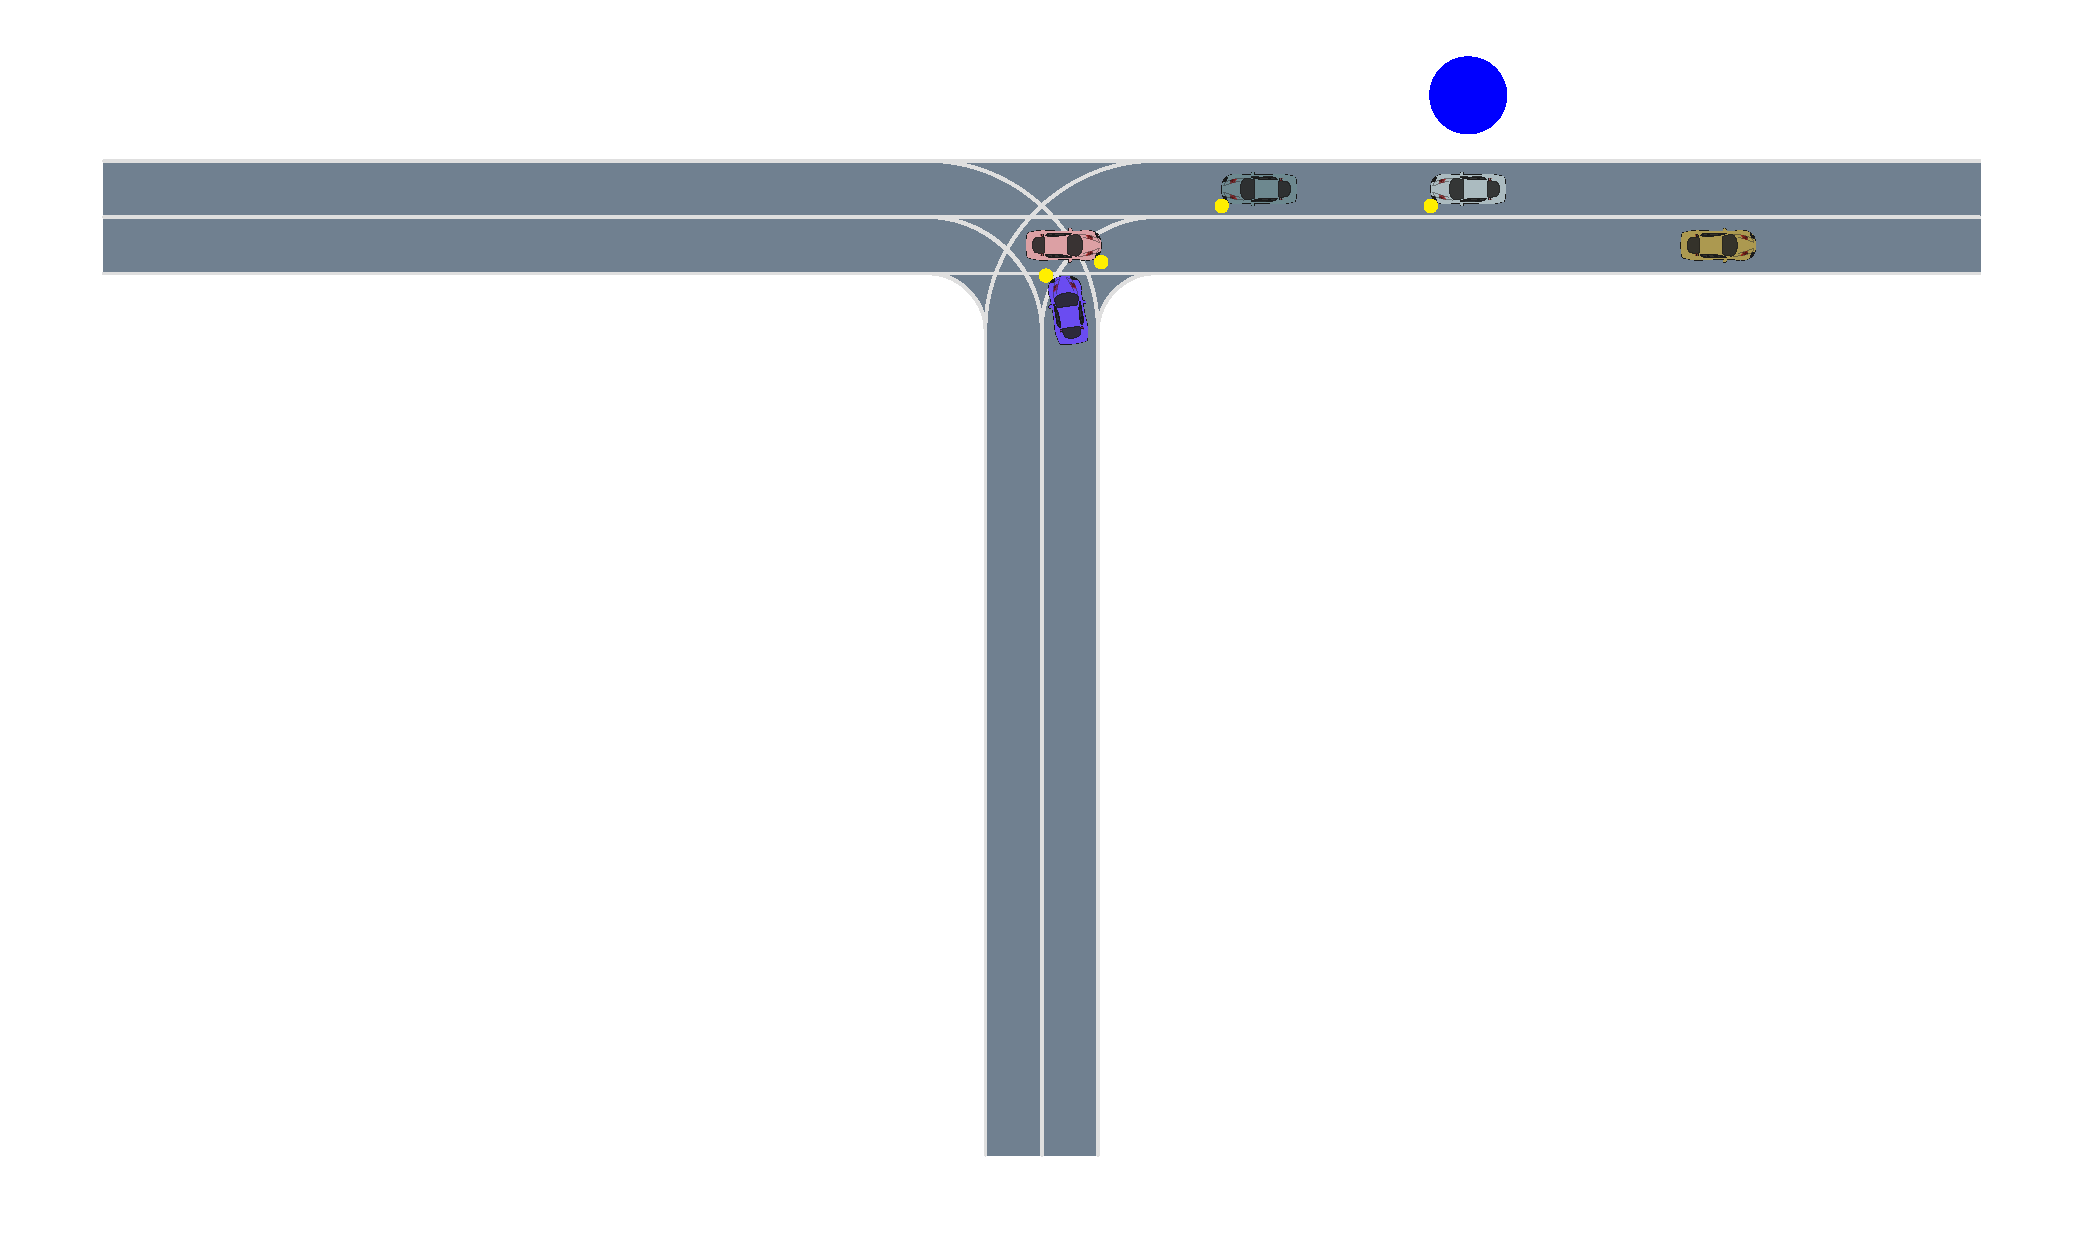
\includegraphics[width=\textwidth, trim={2cm 5cm 1cm 0},clip]{figures/problem_decomposition/f2_27.pdf}
\end{subfigure}
    \caption{Collision in 5-car scenario at timesteps $t=[1,8,27]$}
    \label{fig:five_car_collision2}
    \vspace{-0.2in}
\end{figure}


\section{Discussion}

% Summary
Multi-agent safety validation problems pose a challenge for safety validation algorithms due to the large state and actions paces. In this chapter we made a step toward the scalability of safety validation algorithms to multi-agent settings by applying problem decomposition. We discussed a technique for decomposing a multi-agent system into tractable subproblems and then combining the solutions using the attend, adapt and transfer architecture. 

Using the ground truth of simple multi-agent gridworld problem, we showed that estimates of the probability of failure of the \num{3}-agent system were improved by referencing the probability of failure of the \num{2}-agent system. We then applied the decomposition approach to the T-intersection scenario with \num{4} adversaries. By decomposing the problem into two unique subproblems and recombining their solutions, we were able to approximate the distribution over failures and outperform baseline approaches. 

In addition to the transfer learning literature, our approach to scene decomposition is also similar to the work of \textcite{bouton2019decomposition}. In that work they perform a similar pairwise decomposition to help train a safe driving policy. Each subproblem was solved for the optimal value function and the results were fused with simple aggregated by taking the max or mean. To account for multi-agent interactions, they learned an additive correction factor parameterized by a deep neural network. The A2T approach is more flexible because the combination of subproblem solutions is learned and state dependent. Unlike training an agent to drive, in the safety validation problem the action space scales with the number of agents, which adds an additional challenge to overcome.

In the next chapter we turn away from solving individual safety validation problems and consider the problem of iterative safety validation. We demonstrate that we can gain significant performance and efficiency improvement by storing and reusing safety validation knowledge across systems. 